\documentclass{article}

\usepackage{amsmath} % math stuff
\usepackage{amssymb} % math stuff
\usepackage{array} % equations and stuff
\usepackage{bm} % bold math
%\usepackage{booktabs} % extra table rule options
%\usepackage{caption} % suppressed table numbering; incompatible with revtex, and longtable, I think
\usepackage{comment} % comment environment
%\usepackage{enumitem} % customization of enumeration, itemize, and description
\usepackage[T1]{fontenc} % font encoding for special characters, must also use scalable font package
\usepackage[margin=0.8in]{geometry} % paper sizes and margins (but be careful not to mess up pre-defined pages)
\usepackage{graphicx} % for graphics
%\usepackage{helvet} % default font is the helvetica postscript font
\usepackage{layouts} % print units like widths
\usepackage{lipsum} % lorem ipsum filler text
\usepackage{lmodern} % scalable font?
\usepackage{longtable} % multi-page tables
\usepackage{makecell} % specify line-breaks in table cells
\usepackage{mathrsfs} % math script font
\usepackage{mhchem} % easier chemical formula
\usepackage{microtype} % allows disabling of ligatures
%\usepackage{newcent} % new century schoolbook font
\usepackage{nicefrac}
\usepackage{numprint} % print and format (large) numbers
\usepackage{parskip} % removes paragraph indentation, and adjusts paragraph skip, as well as list items
\usepackage{pdfpages} % add pdf files as pages
%\usepackage{setspace} % adjust text spacing and indents
\usepackage{siunitx} % decimal alignment
\usepackage{subfigure} % divided figures
%\usepackage{tabu} % extra table options
\usepackage{textcomp} % symbols
\usepackage{threeparttablex} % better footnotes with longtable
\usepackage{titling} % title placement
\usepackage{ulem} % strikethrough text
%\usepackage{url} % superceded by hyperref
\usepackage{verbatim} % verbatim environment
\usepackage{xcolor} % colors and color boxes
\usepackage{xspace} % commands that don't eat up white space
\usepackage{hyperref} % links and page setup; should always come last

\hypersetup{
 bookmarks=true,
 colorlinks=true,
 citecolor=blue,
 linkcolor=blue,
 urlcolor=blue,
 pdfstartview={XYZ null null 1.0} % default open view is 100%
}

\DisableLigatures[f,t]{encoding = T1} % disable ff, fi, fl, tt ligatures; without options, it also disables -- = endash
\renewcommand{\arraystretch}{1.0} % extra vertical (and horizontal?) space in tables

% define centered, left- and right-aligned columns with specified widths
\newcommand{\PreserveBackslash}[1]{\let\temp=\\#1\let\\=\temp}
\newcolumntype{C}[1]{>{\PreserveBackslash\centering}p{#1}}
\newcolumntype{L}[1]{>{\PreserveBackslash\raggedright}p{#1}}
\newcolumntype{R}[1]{>{\PreserveBackslash\raggedleft}p{#1}}

\begin{document}

\pagestyle{empty} % don't number pages

% custom title
\begin{center}
{\LARGE Express Riddler}

\vspace{0.15in}

{\Large 23 April 2021}
\end{center}


\section*{Riddle:}

After you intended to make a perfectly circular pancake, the batter has spread out, filling every last corner of your square pan.
(It is unclear why you were using a square pan in the first place.)

To salvage your breakfast, you plan to slice off the corners of your square pancake, giving you something closer to a circle.
The image below shows one such slice you might make.
Each slice must be straight, and no slice can pass through the inscribed blue circle that represents your original desired pancake.

\vspace{0.1in}
\begin{center}
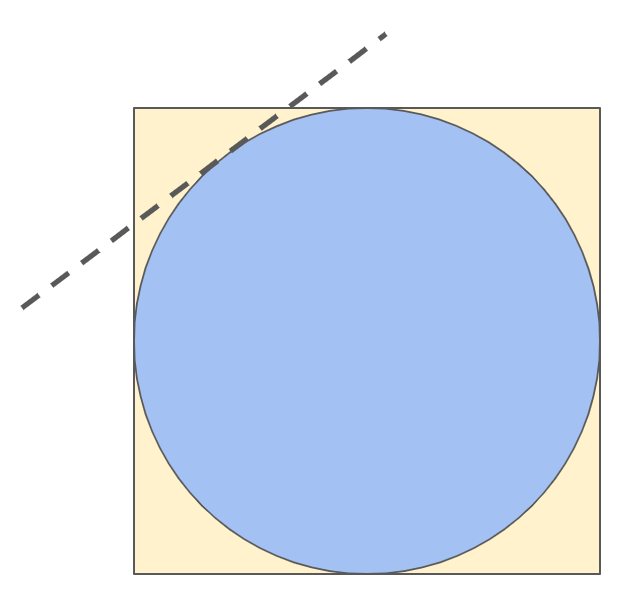
\includegraphics[width=4in]{circle_cut.png}
\end{center}
\vspace{0.1in}

Of course, there's a catch.
You can make at most five slices.
If the blue circle has a radius of 1 unit, what is the minimum possible area your pancake can have after five slices?


\section*{Solution:}

It is intuitive that each cut will be tangent to the circle.
If a cut wasn't tangent, it could be moved inward toward a parallel cut that is tangent, thereby removing more pancake, and leaving a smaller area.
It is also intuitive that the cuts that minimize the area (and best approximate a circle) are those which are equally spaced around the circle.

The square starting shape is essentially 4 cuts already made (and equally spaced, at 90\textdegree\ apart).
There are 5 remaining cuts to be distributed in the 4 corner sections.
The final intuition I use to solve this problem is that the slices which minimize the area are those that are as evenly distributed among the corners as possible.
That is, the corner with the most slices has at most 1 more slice than the corner with the fewest slices.
In this case, that means that there are 3 corners with 1 slice, and 1 corner with 2 slices.

For the first three corners (say upper left, bottom left, and bottom right), equal spacing means these slices will be at 45\textdegree\ relative to the existing slices, and will be tangent to the circle at 135\textdegree, 225\textdegree, and 315\textdegree\ (measured counterclockwise from the right).
The last corner (upper right) will have 2 slices, and will be tangent to the circle at 30\textdegree\ and 60\textdegree.
The only step left is determining the area.
The resulting shape is a nonagon, which can be subdivided into 18 right triangles, each with a side length equal to the radius (1).
Six of the triangles (in the upper right) have 15\textdegree\ angles, and the remaining 12 have 22.5\textdegree\ angles.
Calculating the area of these triangles gives a solution of
\fcolorbox{red}{white}{$\bm{6\sqrt{2}-3\sqrt{3}}$}\,.
This is approximately 3.289, and is only 4.7\% away from the ideal area of $\pi$.



\end{document}